\vspace{-0.1cm}
\section{Experiments}\label{sec:exp}
\vspace{-0.1cm}
%\subsection{Case Study}
\begin{figure}
\begin{minipage}{0.63\textwidth}
%\begin{wraptable}{r}{0.5\textwidth}
%\begin{table}[t]
%\fontsize{10}{6}\selectfont
%\setlength\tabcolsep{4pt}
\centering
\captionof{table}{The discrete objectives (Eq.~\ref{eq:def_CO}) and their relaxations (Eq.~\ref{eq:relax}) for the three problems to be studied.}
\label{exp:tab_case_study}
\resizebox{\textwidth}{!}{\begin{tabular}{@{}ccc@{}}
\toprule
\multirow{2.5}{*}{MC} & Discrete Obj. & $\max_{X}  \sum_{1\leq i\leq n} X_i  \quad \quad \text{s.t.} \quad  (i, j) \in E\;\text{if}\;{X_i, X_j = 1} $ \\ \cmidrule(l){2-3} 

 & Relaxation & $l_{\text{MC}}(\theta;G) \triangleq - (\beta+1)\sum_{(i,j)\in E} \bar{X}_i \bar{X}_j + \frac{\beta}{2} \sum_{i \neq j} \bar{X}_i \bar{X}_j$ \\ \midrule
 
\multirow{2.5}{*}{MVC} & Discrete Obj. & $\min_{X} \sum_{1 \leq i \leq n} X_i \quad \quad \text{s.t.} \quad  X_i + X_j \geq 1\;\;\text{if}\;(i,j)\in E \ $ \\ \cmidrule(l){2-3} 

 & Relaxation & $l_{\text{MVC}}(\theta;G) \triangleq \sum_{1\leq i \leq n} \bar{X}_i +\beta \sum_{(i,j) \in E} (1-\bar{X}_i) (1-\bar{X}_j)$ \\ \midrule
 
% \multirow{2.5}{*}{MDS} & Formulation & $\min_{X} \sum_{1 \leq i \leq n} X_i \quad \quad \text{s.t.} \quad  \  (1-X_i) \prod_{j \in \mathcal{N}(i)} (1-X_j) \leq 0$ \;\text{if}\; $i \in V$\\ \cmidrule(l){2-3}

%  & Loss Design & $l_{\text{MDS}}(\theta;G) \triangleq \sum_{1 \leq i \leq n} \bar{X}_i + \beta \sum_{i\in V} (1-\bar{X}_i)\prod_{j \in \mathcal{N}(i)}(1-\bar{X}_j)$ \\ \midrule
 
\multirow{2.5}{*}{MIS} & Discrete Obj. & $\max_{X} \sum_{1 \leq i \leq n} X_i \quad \quad \text{s.t.} \quad  X_iX_j = 0 \;\text{if}\; (i,j) \in E$ \\ \cmidrule(l){2-3} 

 & Relaxation & $l_{\text{MIS}}(\theta;G) \triangleq -\sum_{1 \leq i \leq n} \bar{X}_i + \beta \sum_{(i,j) \in E} \bar{X_i} \bar{X_j}$ \\ \bottomrule
\end{tabular}}
%\end{wraptable}
%\end{table}
\end{minipage}
\hfill
\begin{minipage}{0.34\textwidth}
%\begin{figure}
%\begin{center}
\caption{Performance v.s. hyper-parameter $\rho$ of the RB model}
\vspace{-0.1cm}
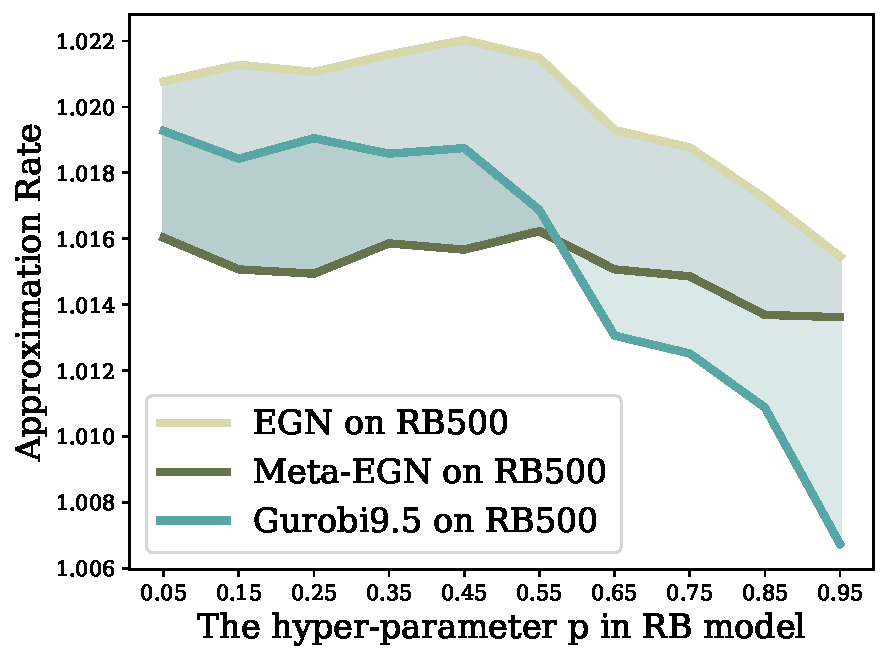
\includegraphics[width=0.92\textwidth]{iclr2023/img/exp/difficulty_mvc.pdf}
%\end{center}
\vspace{-0.5cm}
\label{fig:difficulty_rb}
%\end{figure}
\end{minipage}
\end{figure}

We study three CO problems, namely \emph{max clique (MC)} to find the largest set of nodes where each pair of nodes are connected,  \emph{minimum vertex covering (MVC)} to find the smallest set of nodes that every edge is connected to at least one nodes in the set, and  \emph{max independent set (MIS)} to find the largest set where any two vertices in the set are not adjacent. Their objectives (Eq.~\ref{eq:def_CO}) and relaxations (Eq.~\ref{eq:relax})  are listed in Table~\ref{exp:tab_case_study}. For the detailed derivation, see Appendix ~\ref{sec:app_experiment_details}.

%Also, if learning-based methods are fine-tuned based on the test instance, we highlight them with ``f-t''. We only consider

%\end{table}



\vspace{-0.1cm}
\subsection{Settings}\label{sec:settings}
\vspace{-0.1cm}
% \begin{wrapfigure}{r}{0.42\textwidth}
% \vspace{-1cm}
%   \begin{center}
%     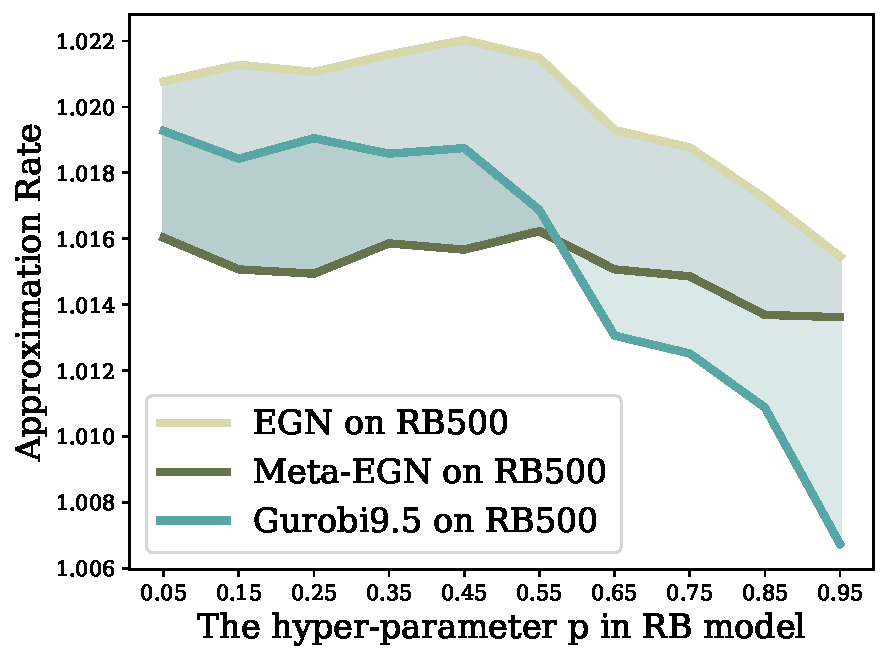
\includegraphics[width=0.42\textwidth]{iclr2023/img/exp/difficulty_mvc.pdf}
%   \end{center}
%   \vspace{-0.5cm}
%   \caption{Cross-Difficulty of RB on MVC}
%   \label{fig:difficulty_rb}
% \end{wrapfigure}

\textbf{Datasets:} We conduct experiments on the MC and MVC problems over three real datasets Twitter~\citep{leskovec2014snap}, COLLAB and IMDB~\citep{yanardag2015deep} and two synthetic datasets with $200$ and $500$ nodes generated by the RB model~\citep{xu2007benchmarks}. We name them RB200 and RB500, respectively. We make RB200 and RB500 extremely hard by setting a small hyper-parameter $\rho=0.25$ of the RB model~\citep{xu2007benchmarks}. The difficulty-$\rho$ relationship on the MVC problem with $500$ vertices is shown in Fig.~\ref{fig:difficulty_rb}, where the models are pre-trained on the RB graphs with uniformly sampled $\rho \in [0.3,1.0]$ and tested on different RB graphs generated with single $\rho$'s. We keep all the other hyper-parameters the same. As $\rho$ increases, Meta-EGN and Gurobi9.5 all tend to achieve better performance. Meta-EGN could outperform Gurobi9.5 in hard instances $\rho \in (0,0.55]$ while remaining a gap on the easy ones.
To verify performances for data-scale generalization, we also generate large-graph datasets RB1000, RB2000, and RB5000 with $\rho=0.25$. As for the MIS problem, random-regular graphs (RRGs) are often used as benchmarks because they are challenging. Our experiments also use RRGs by following the settings of ~\citep{schuetz2022combinatorial} with the node number ranging from $10^2$ to $10^5$ and the node degree selected from the set $\mathcal{D}=\{3,7,10,20\}$. Here, node degree equaling 20 is the hardest setting~\citep{angelini2022cracking}. A summary of these datasets is in Table.~\ref{tab:dataset_details} in Appendix.

\textbf{Data Splitting \& The Evaluation Metric:} For the real datasets, training/validation/test instances are randomly divided with the ratio of 8:1:1; For RB200 and RB500, $2000/100/100$ graphs are generated for training/validation/test instances; For RB1000, RB2000, RB5000, we generate $100$ test instances. As to RRG datasets, the training set contains $3000$ RRGs, of which each has $1000$ nodes and the node degree is uniformly sampled from $\mathcal{D}$. We generate 30/20 graphs for each node degree configuration in $\mathcal{D}$ for validation/test. Our evaluation metric uses the approximation rate (ApR). All results are summarized based on $5$ times independent experiments with different random seeds.%For Gurobi9.5, we set the time budget the same as that required in learning-based methods.  %which calculates the ratio between the algorithm's answer and the optimal solution. For Gurobi9.5, we set the time budget the same as that required in learning-based methods. 

%the training set that contains $3000$ graphs with $1000$ vertices, we use the same emthods to generate the validation set with $30$ graphs, for each testing dataset with each scale and degree we generate $20$ different testing instances, following the setting of ~\cite{schuetz2022combinatorial}. 
 %and list the actual time usage next to its performance.

\begin{table}[t]

%\fontsize{7}{5}\selectfont
%\setlength\tabcolsep{3pt}
    \centering
    \begin{minipage}{1.00 \linewidth}
    \caption{ApR (time: second/graph) on the MC problem. ApR is the larger the better. `report' denotes the reported performance in ~\cite{karalias2020erdos}, `re-impl' denotes re-implementation, `f-t' stands for fine-tune. Pareto-optimal results are in bold.}
    \vspace{-0.2cm}
     \label{tab:mc_performance}
     \centering
    \resizebox{1.0\textwidth}{!}{\begin{tabular}{@{}cccccc@{}}
\toprule
                    & Twitter              & COLLAB               & IMDB         & RB 200 & RB 500 \\ \midrule
EGN (report)        & 0.924 \hspace{-0.3mm}$\pm$\hspace{-0.3mm} 0.133 (0.17) & 0.982 \hspace{-0.3mm}$\pm$\hspace{-0.3mm} 0.063 (0.10) & 1.000 (0.08)  &   -     &    -    \\
EGN (re-impl)     & 0.926 \hspace{-0.3mm}$\pm$\hspace{-0.3mm} 0.113(0.17)  & 0.982 \hspace{-0.3mm}$\pm$\hspace{-0.3mm} 0.069 (0.10) & 1.000 (0.08) &     0.820 \hspace{-0.3mm}$\pm$\hspace{-0.3mm} 0.188 (0.26)  &  0.829 \hspace{-0.3mm}$\pm$\hspace{-0.3mm} 0.192 (0.29)       \\
EGN (re-impl) f-t & 0.949 \hspace{-0.3mm}$\pm$\hspace{-0.3mm} 0.102(0.49)  & 0.986 \hspace{-0.3mm}$\pm$\hspace{-0.3mm} 0.060(0.27)    & 1.000 (0.20)  &    0.846 \hspace{-0.3mm}$\pm$\hspace{-0.3mm} 0.180 (0.81)    &  0.864 \hspace{-0.3mm}$\pm$\hspace{-0.3mm} 0.181 (0.89)      \\
RUN-CSP          & 0.909 \hspace{-0.3mm}$\pm$\hspace{-0.3mm} 0.145 (0.21) & 0.912 \hspace{-0.3mm}$\pm$\hspace{-0.3mm} 0.188 (0.14) & 0.823 \hspace{-0.3mm}$\pm$\hspace{-0.3mm} 0.191 (0.11) & 0.858 \hspace{-0.3mm}$\pm$\hspace{-0.3mm} 0.731 (2.05) & 0.748 \hspace{-0.3mm}$\pm$\hspace{-0.3mm} 0.689 (2.16) \\
Meta-EGN            & \textbf{0.976 \hspace{-0.3mm}$\pm$\hspace{-0.3mm} 0.048(0.17)}  & 0.988 \hspace{-0.3mm}$\pm$\hspace{-0.3mm} 0.059 (0.10) & 1.000 (0.08) &    \textbf{0.834 \hspace{-0.3mm}$\pm$\hspace{-0.3mm} 0.178 (0.26)}     &    \textbf{0.834 \hspace{-0.3mm}$\pm$\hspace{-0.3mm} 0.198 (0.29)}    \\
Meta-EGN f-t        & 0.990 \hspace{-0.3mm}$\pm$\hspace{-0.3mm} 0.028(0.49)  & 0.993 \hspace{-0.3mm}$\pm$\hspace{-0.3mm} 0.038 (0.27) & 1.000 (0.20) &    \textbf{0.874  \hspace{-0.3mm}$\pm$\hspace{-0.3mm} 0.169 (0.81)}    &    \textbf{0.878 \hspace{-0.3mm}$\pm$\hspace{-0.3mm} 0.181 (0.89)}    \\ \midrule
Toenshoff-Greedy & \textbf{0.917 \hspace{-0.3mm}$\pm$\hspace{-0.3mm} 0.126 (0.08)}  & 0.969 \hspace{-0.3mm}$\pm$\hspace{-0.3mm} 0.087 (0.06) & 0.987 \hspace{-0.3mm}$\pm$\hspace{-0.3mm} 0.050 (1e-3) & 0.786 \hspace{-0.3mm}$\pm$\hspace{-0.3mm} 0.195 (2.25) & 0.793 \hspace{-0.3mm}$\pm$\hspace{-0.3mm} 0.202 (2.38) \\ \midrule

Gurobi9.5 ($\leq$0.20s)   & 0.737 \hspace{-0.3mm}$\pm$\hspace{-0.3mm} 0.267 (0.17)&  \textbf{0.871 \hspace{-0.3mm}$\pm$\hspace{-0.3mm} 0.242 (0.04)} & \textbf{1.000 (1e-3)}  &  -    &    -    \\
Gurobi9.5 ($\leq$1.00s)   & \textbf{1.000 (0.37)}& 0.979 \hspace{-0.3mm}$\pm$\hspace{-0.3mm} 0.117 (0.06)& 1.000 (1e-3)  &   -   &    -    \\
Gurobi9.5 ($\leq$2.50s)   &1.000 (0.37)& 0.997 \hspace{-0.3mm}$\pm$\hspace{-0.3mm} 0.036 (0.06) & 1.000 (1e-3)  &  0.667 \hspace{-0.3mm}$\pm$\hspace{-0.3mm} 0.188 (2.10)    &    0.663 \hspace{-0.3mm}$\pm$\hspace{-0.3mm} 0.188 (2.41)    \\
Gurobi9.5 ($\leq$4.00s)   & 1.000 (0.37)& \textbf{1.000 (0.06)} & 1.000 (1e-3)  &  0.755 \hspace{-0.3mm}$\pm$\hspace{-0.3mm} 0.225 (3.96) &    0.742 \hspace{-0.3mm}$\pm$\hspace{-0.3mm} 0.213 (3.88)    \\
 \bottomrule
\end{tabular}}

    \end{minipage}
   \begin{minipage}{1.00 \linewidth}
   \vspace{2mm}
    \caption{ApR (time: second/graph)  on the MVC problem. ApR is the smaller the better.. `f-t' stands for one-step fine-tune. Pareto-optimal results are in bold.}
    \vspace{-0.2cm}
     \label{tab:mvc_performance}
     \centering
     \resizebox{1.0\textwidth}{!}{\begin{tabular}{@{}cccccc@{}}
\toprule
                  & Twitter             & COLLAB                & IMDB                 & RB 200 & RB 500 \\ \midrule
EGN               & 1.033 \hspace{-0.3mm}$\pm$\hspace{-0.3mm} 0.023(0.29) & 1.013 \hspace{-0.3mm}$\pm$\hspace{-0.3mm} 0.022 (0.15)  & 1.000 (0.08)             &    1.031 \hspace{-0.3mm}$\pm$\hspace{-0.3mm} 0.004 (0.26)    &    1.021 \hspace{-0.3mm}$\pm$\hspace{-0.3mm} 0.002 (0.48)    \\
EGN f-t           & 1.028 \hspace{-0.3mm}$\pm$\hspace{-0.3mm} 0.021(0.80) & 1.008 \hspace{-0.3mm}$\pm$\hspace{-0.3mm} 0.015 (0.38)  & 1.000 (0.32)             &    1.030 \hspace{-0.3mm}$\pm$\hspace{-0.3mm} 0.005 (0.80)    &   1.021 \hspace{-0.3mm}$\pm$\hspace{-0.3mm} 0.002 (1.59)    \\
RUN-CSP           &         1.180 \hspace{-0.3mm}$\pm$\hspace{-0.3mm} 0.435 (0.16)            &            1.208 \hspace{-0.3mm}$\pm$\hspace{-0.3mm} 0.198 (0.19)           &          1.188 \hspace{-0.3mm}$\pm$\hspace{-0.3mm} 0.178 (0.08)            &   1.124 \hspace{-0.3mm}$\pm$\hspace{-0.3mm} 0.001 (0.28)     &   1.062 \hspace{-0.3mm}$\pm$\hspace{-0.3mm} 0.005 (1.65)     \\
Meta-EGN          & 1.019 \hspace{-0.3mm}$\pm$\hspace{-0.3mm} 0.017(0.29) & 1.003 \hspace{-0.3mm}$\pm$\hspace{-0.3mm} 0.010 (0.15) & 1.000 (0.08)             &    \textbf{1.028 \hspace{-0.3mm}$\pm$\hspace{-0.3mm} 0.005 (0.26)}    &    \textbf{1.016 \hspace{-0.3mm}$\pm$\hspace{-0.3mm} 0.002 (0.48)}    \\
Meta-EGN f-t      & 1.017 \hspace{-0.3mm}$\pm$\hspace{-0.3mm} 0.017(0.80) & 1.002 \hspace{-0.3mm}$\pm$\hspace{-0.3mm} 0.010 (0.38) & 1.000 (0.32)             &   1.027 \hspace{-0.3mm}$\pm$\hspace{-0.3mm} 0.006 (0.80)     &    1.016 \hspace{-0.3mm}$\pm$\hspace{-0.3mm} 0.002 (1.59)    \\ \midrule
Greedy            &     1.014 \hspace{-0.3mm}$\pm$\hspace{-0.3mm} 0.014 (1.95)                &           1.209 \hspace{-0.3mm}$\pm$\hspace{-0.3mm} 0.198 (1.79)            &            1.180 \hspace{-0.3mm}$\pm$\hspace{-0.3mm} 0.077 (0.02)          &    1.124 \hspace{-0.3mm}$\pm$\hspace{-0.3mm} 0.002 (5.02)    &    1.062 \hspace{-0.3mm}$\pm$\hspace{-0.3mm} 0.005 (15.59)    \\ \midrule
Gurobi9.5 ($\leq$0.25s) & \textbf{1.028 \hspace{-0.3mm}$\pm$\hspace{-0.3mm} 0.054 (0.09)} &  1.002 \hspace{-0.3mm}$\pm$\hspace{-0.3mm} 0.010 (0.10)  &    \textbf{1.000 (0.01)}   &   -     &   -     \\
Gurobi9.5 ($\leq$0.50s) & 1+1e-3 \hspace{-0.3mm}$\pm$\hspace{-0.3mm} 0.001 (0.13) &  \textbf{1.000 (0.10)}   &   1.000 (0.01)   &   -     &    -    \\
Gurobi9.5 ($\leq$1.00s) & \textbf{1.000 (0.13)} &  1.000 (0.10)   &   1.000 (0.01)   &    \textbf{1.011 \hspace{-0.3mm}$\pm$\hspace{-0.3mm} 0.003 (0.63)}    &   1.019 \hspace{-0.3mm}$\pm$\hspace{-0.3mm} 0.003 (0.69)     \\
Gurobi9.5 ($\leq$2.00s) & 1.000 (0.13) &  1.000 (0.10)   &   1.000 (0.01)   &   \textbf{1.008 \hspace{-0.3mm}$\pm$\hspace{-0.3mm} 0.002 (1.16)}     &    1.019 \hspace{-0.3mm}$\pm$\hspace{-0.3mm} 0.003 (1.68)    \\ \bottomrule
\end{tabular}}
    
     
   \end{minipage}
 \vspace{-4mm}
\end{table}

\textbf{Baselines:} Our baselines include unsupervised learning methods, heuristics, and traditional CO solvers. 
For the MC and MVC problems, we take our direct baseline EGN~\citep{karalias2020erdos}, and also take RUN-CSP~\citep{toenshoff2021graph} as another baseline. %As RUN-CSP is designed for constraint satisfaction problems with only two variables in each constraint, we don't consider it in the MDS problem which normally has more than two variables in each constraint. 
We do not consider other learning-based methods because they generally perform worse than EGN~\citep{karalias2020erdos}. %have already been shown to have huge performance gaps from EGN.
As to the heuristics, we use greedy algorithms as heuristic baselines. For traditional CO solvers, we compare against the best commercial CO problem solver Gurobi9.5~\citep{Gurobi} via converting the problems into integer programming form. We track the time $t$ that the models use from the start of inferring to the end of rounding to output feasible solutions. We set this time $t$ as the time budget of Gurobi9.5 for purely solving the integer programming, and list the actual time usage of Gurobi9.5 which includes pre-processing plus $t$.
As to the MIS problem, we take PI-GNN~\citep{schuetz2022combinatorial} and EGN~\cite{karalias2020erdos} as the learning-based baselines. We take the random greedy algorithm (RGA) and degree-based greedy algorithm (DGA) as introduced in ~\cite{angelini2019monte} as the heuristic baselines. When we consider fine-tuning EGN and \proj over a test instance, we use 1-step gradient descent as fine-tuning.

\textbf{Implementation:}
For the MC and MVC problems, we use 4-layer GIN~\citep{xu2018powerful} as the backbone network for both meta-EGN and EGN. We use 1e-3 as both the outer learning rate ($\gamma$) of Meta-EGN and the learning rate of EGN. Here, the backbone and the learning rate are the same as those in~\citep{karalias2020erdos}. For the MIS problem, we use $6$-layer GIN. The outer learning rate  ($\gamma$) of Meta-EGN and the learning rate of EGN are set as 1e-4. The inner learning rate ($\alpha$) of \proj is always set as 5e-5. We run all experiments by using a Xeon(R) Gold 6248 CPU with 26 threads and a Quadro RTX $6000$ GPU. All codes run on the PyTorch platform~\citep{NEURIPS2019_9015}. For more details, see Appendix.~\ref{sec:app_experiment_details}.

\textbf{Overcoming the limited expressive power of GNNs:} GNNs are known with limited expressive power~\citep{xu2018powerful,morris2019weisfeiler}. Specifically, over RRGs, the GIN backbone will associate each node with the same representation, unless node representations are initialized not equally. To keep a fair comparison, for the MC and MVC problem, we follow~\cite{karalias2020erdos} and adopt the initialization based on a single random node seed (one selected node is initialized as 1, others as 0). We use 8 single random node seeds for EGN and \proj in the experiments of Sec.~\ref{sec:in-dis} and report the best among the 8 trials. We try different numbers of random node seeds in the experiments of  Sec.~\ref{sec:out-dis}. For the large-scale MIS problem studied in Sec.~\ref{sec:MIS}, we find such single node initialization is too local to generate valid global solutions. So, we adopt initialization based on the solutions of greedy algorithms DGA (for Figs.~\ref{fig:mis},\ref{fig:dynamic}) and RGA (for Fig.~\ref{fig:mis_ga}). Then, EGN and \proj can be viewed as learning heuristics to improve the greedy solutions. Note that learning heuristics to tune these solutions is non-trivial~\citep{andrade2012fast,rahman2017local}. %.because there is no explicit local tuning approaches to MIS problems.   

%whose results are shown in Figs.~\ref{fig:mis},\ref{fig:dynamic},\ref{fig:mis_ga},

%which always fails the 


%All of the experiments are carried out on the same server with 2 Intel(R) Xeon(R) Gold 6248 CPUs, $1000GB$ RAM in total. In each experiment we take $26$ processes and run on a single Quadro RTX $6000$ GPU. Codes run on the PyTorch~\citep{NEURIPS2019_9015} platform and the PyTorch geometric framework~\citep{Fey/Lenssen/2019}. For more details, see Appendix.~\ref{}.

%The backbone network shares exactly the same structure as that used in the MC problem in ~\citep{karalias2020erdos}.
%, which keeps the same setting in ~\citep{karalias2020erdos} , which keeps the same setting in ~\citep{karalias2020erdos}

%The inner learning rate of Meta-EGN is set as 5e-5.



\begin{table}[t]
%\fontsize{6}{7}\selectfont
%\setlength\tabcolsep{1.5pt}
    \centering
    %\begin{minipage}{1.00 \linewidth}
    %\caption{Scale generalization performance on the max clique (MC) problem. Optimal solutions are generated via Gurobi9.5 with the time limit $3000$ seconds. Approximation rate larger than $1$, highlighted by $^*$, indicates the model outperforms Gurobi9.5 solver with $3000$s time budget.}
        \caption{Scale generalization performance on the MC and MVC problems. ApR is the larger the better for MC while the smaller the better for MVC. All the models are trained on RB500 training data. `Fast/Medium/Accurate' denotes GNNs (without fine-tuning) using $1/4/8$ random single node seed(s) per testing instance. `Fine-tuning' use 1-step Fine-tuning the best trial among the 8 node seed(s). `Gap' represents the averaged gap defined as $c\times($\# of nodes in the optimal solution - \# of nodes by the given method$)$ where $c=1$ for MC and $c=-1$ for MVC. `Rank' is the average rank of solutions among the three methods. Optimal solutions are generated via Gurobi9.5 with a time limit $3000$ seconds. Approximation rate for MC larger than $1$, highlighted by $^*$, indicates the model outperforms Gurobi9.5 solver with $3000$s time budget. Pareto-optimal results are in bold.}
    
     \label{tab:mc_generaliztaion_scale}
     \vspace{-0.2cm}
     \centering
\resizebox{1.0\textwidth}{!}{\begin{tabular}{@{}ccc|ccc|ccc|ccc|ccc@{}}
\toprule
& \multirow{2}{*}{Dataset} & \multirow{2}{*}{Method} & \multicolumn{3}{c|}{Fast (1)} & \multicolumn{3}{c|}{Medium (4)} & \multicolumn{3}{c|}{Accurate (8)} & \multicolumn{3}{c}{Fine-tune} \\
& &  & ApR(s/g) & Gap & Rank & ApR(s/g) & Gap & Rank & ApR(s/g) & Gap & Rank & ApR(s/g) & Gap & Rank \\ \midrule
\multirow{10}{*}{MC} & \multirow{3}{*}{RB1000} &  EGN & 0.6462±0.282(0.05) & 11.48 & 2.406 & 0.8433±0.229(0.17) & 6.47 & 2.237 & 0.9099±0.205(0.33) & 4.86 & 2.025 & 0.9631±0.186(0.98) & 4.13 & 1.693 \\
 && Meta-EGN & 0.7692±0.276(0.05) & 8.57 & 1.943 & \textbf{0.9388±0.196(0.17)} & \textbf{4.61} & \textbf{1.543} & \textbf{0.9408±0.205(0.33)} & \textbf{4.97} & \textbf{1.581} & \textbf{0.9745±0.195(0.98)} & \textbf{4.01} & \textbf{1.625} \\
 & & Gurobi9.5 & \textbf{0.8851±0.197(6.11)} & \textbf{5.08} & \textbf{1.650} & 0.8851±0.197(6.18) & 5.08 & 2.218 & 0.8851±0.197(6.48) & 5.08 & 2.393 & 0.8851±0.197(7.01) & 5.08 & 2.681 \\ \cmidrule(l){2-15} 
& \multirow{3}{*}{RB2000} & EGN & 0.6793±0.290(0.10) & 12.38 & 2.408 & 0.8968±0.184(0.29) & 5.23 & 2.136 & 0.9454±0.160(0.58) & 3.81 & 2.208 & 0.9714±0.154(2.03) & 3.61 & 1.983 \\
& & Meta-EGN & 0.8077±0.114(0.10) & 8.13 & 1.991 & \textbf{0.9783±0.157(0.29)} & \textbf{3.48} & \textbf{1.591} & \textbf{0.9958±0.146(0.58)} & \textbf{1.28} & \textbf{1.466} & \textbf{1.0112±0.134(2.03)}$^*$ & \textbf{0.55} & \textbf{1.483} \\
& & Gurobi9.5 & \textbf{0.9510±0.145(24.14)} & \textbf{3.01} & \textbf{1.600} & 0.9510±0.145(24.56) & 3.01 & 2.091 & 0.9510±0.145(25.01) & 3.01 & 2.325 & 0.9510±0.145(25.66) & 3.01 & 2.533 \\ \cmidrule(l){2-15}
& \multirow{4}{*}{RB5000} & EGN & 0.9603±0.159(0.33) & 2.42 & 2.130 & 1.0203±0.139(1.02)$^*$ & -1.26 & 2.060 & 1.0272±0.140(2.50)$^*$ & -1.68 & 1.980 & 1.0475±0.188(9.66)$^*$ & -2.86 & 1.970 \\
& & Meta-EGN & \textbf{1.0288±0.138(0.33)}$^*$ & \textbf{-1.62} & \textbf{1.820} & \textbf{1.0684±0.233(1.02)}$^*$ & \textbf{-4.02} & \textbf{1.820} & \textbf{1.0727±0.234(2.50)}$^*$ & \textbf{-4.42} & \textbf{1.790} & \textbf{1.0778±0.233(9.66)}$^*$ & \textbf{-4.72} & \textbf{1.710} \\
& & Gurobi9.5 & 1.0000(201.55) & 0.00 & 2.050 & 1.0000(202.36) & 0.00 & 2.120 & 1.0000(205.64) & 0.00 & 2.230 & 1.0000(214.35) & 0.00 & 2.320 \\
& & Gurobi9.5 & 1.0000(3000) & 0.00 & - & 1.0000(3000) & 0.00 & - & 1.0000(3000) & 0.00 & - & 1.0000(3000) & 0.00 & - \\ %\bottomrule
%\end{tabular}}
     %\vspace{-0.2cm}
     %\centering
     %\fontsize{6}{7}\selectfont
%\setlength\tabcolsep{1pt}
%\resizebox{1.0\textwidth}{!}{\begin{tabular}{@{}cc|ccc|ccc|ccc|ccc@{}}
%\toprule
%\multirow{2}{*}{Dataset} & \multirow{2}{*}{Method} & \multicolumn{3}{c|}{Fast (1)} & \multicolumn{3}{c|}{Medium (4)} & \multicolumn{3}{c|}{Accurate (8)} & \multicolumn{3}{c}{Fine-tune} \\
 %&  & ApR & Gap & Rank & ApR & Gap & Rank & ApR & Gap & Rank & ApR & Gap & Rank \\ 
 \midrule
\multirow{10}{*}{MVC} & \multirow{3}{*}{RB1000} & EGN & 1.0161±0.0048(0.20) & 16.46 & 2.250 & 1.0135±0.0013(0.72) & 13.73 & 1.920 & 1.0138±0.0013(1.37) & 13.29 & 1.860 & 1.0138±0.0013(3.05) & 13.28 & 1.960 \\
&& Meta-EGN & 1.0145±0.0016(0.20) & 14.81 & 1.935 & \textbf{0.0131±0.0012(0.72)} & \textbf{13.40} & \textbf{1.700} & \textbf{1.0125±0.0012(1.37)} & \textbf{12.75} & \textbf{1.545} & \textbf{1.0124±0.0012(3.05)} & \textbf{12.69} & \textbf{1.455} \\
&& Gurobi9.5 & \textbf{1.0143±0.0018(1.92)} & \textbf{14.58} & \textbf{1.835} & 1.0143±0.0018(2.58) & 14.58 & 2.380 & 1.0143±0.0018(3.08) & 14.58 & 2.595 & 1.0143±0.0018(4.96) & 14.58 & 2.585 \\ \cmidrule(l){2-15} 
&\multirow{3}{*}{RB2000} &  EGN & 1.0114±0.0026(0.34) & 22.02 & 2.350 & 1.0096±0.0008(1.32) & 18.57 & 1.765 & 1.0094±0.0007(2.69) & 18.17 & 1.765 & 1.0093±0.0007(6.27) & 17.98 & 1.890 \\
& & Meta-EGN & \textbf{0.0103±0.0015(0.34)} & \textbf{19.94} & \textbf{1.740} & \textbf{1.0095±0.0008(1.32)} & \textbf{18.41} & \textbf{1.635} & \textbf{1.0092±0.0007(2.69)} & \textbf{17.82} & \textbf{1.510} & \textbf{1.0090±0.0006(6.27)} & \textbf{17.38} & \textbf{1.360} \\
& & Gurobi9.5 & 1.0104±0.0010(5.63) & 20.18 & 2.910 & 1.0104±0.0010(6.65) & 20.18 & 2.600 & 1.0104±0.0010(8.04) & 20.18 & 2.725 & 1.0104±0.0010(13.24) & 20.18 & 2.750 \\ \cmidrule(l){2-15} 
&\multirow{3}{*}{RB5000} & EGN & 1.0071±0.0014(1.01) & 34.19 & 2.170 & 1.0064±0.0004(3.99) & 30.83 & 1.985 & 1.0062±0.0004(7.95) & 29.87 & 1.865 & 1.0062±0.0004(18.41) & 29.68 & 1.960 \\
& & Meta-EGN & \textbf{1.0067±0.0005(1.01)} & \textbf{32.51} & \textbf{2.045} & \textbf{1.0062±0.0005(3.99)} & \textbf{29.96} & \textbf{1.600} & \textbf{1.0061±0.0004(7.95)} & \textbf{29.44} & \textbf{1.555} & \textbf{1.0060±0.0003(18.41)} & \textbf{29.15} & \textbf{1.470} \\
& & Gurobi9.5 & 1.0066±0.0006(24.60) & 31.88 & 1.785 & 1.0066±0.0006(28.72) & 31.88 & 2.415 & 1.0066±0.0006(32.16) & 31.88 & 2.580 & 1.0066±0.0006(42.62) & 31.88 & 2.570 \\ \bottomrule
\end{tabular}}
    %\end{minipage}
    \vspace{-3mm}
\end{table}

\subsection{\proj boosts the performance without distribution shifts}\label{sec:in-dis}

%To prove Meta-EGN's improvement in performance, we show the experiment results of the MC in Table~\ref{tab:mc_performance}, the MVC in Table~\ref{tab:mvc_performance}. %and the MDS in Table~\ref{tab:mds_performance} (See Appendix). 
We first compare the performances of different methods when the datasets used for training and testing are from the same distribution. Table~\ref{tab:mc_performance} and Table~\ref{tab:mvc_performance} show the results for the MC problem and the MVC problem respectively. 
In both problems and across the five datasets, Meta-EGN significantly outperforms EGN and RUN-CSP, both before and after the fine-tuning step. In comparison with the traditional CO solvers, Meta-EGN narrows the gap from Gurobi9.5 on those real small graphs. For RB graphs, Meta-EGN outperforms Gurobi9.5 for the MC problem. For the MVC problem, Meta-EGN outperforms Gurobi9.5 on RB500. 

We notice that both EGN and Meta-EGN perform generally well on the MC problem while not as competitive on the MVC problem. This results from the initialization of GNN inputs. The MC problem outputs clusters that are more local while MVC asks for global assignments, which makes such single-seed-based initialization less fit for the MVC problem. %In the later MIS problem, we adopt    

%to reason the local relationship to form large clusters which naturally suits for the initialization design in the models(randomly set a vertex as $1$), while the MVC and MDS problems require to reason the global assignments and relationships between distant vertices on large graphs, where the random initialization seeds might potentially limit the performance.
%The time limit for Gurobi9.5 is set the same as the learning-based methods, the actual time usage is below the approximation rate.
\begin{table}[t]
%\fontsize{7}{6}\selectfont
%\setlength\tabcolsep{3pt}
\centering
\caption{Generalization performance from Twitter to RB2000 on the MC and MVC problems. Pareto-optimal results are in bold.}     \label{tab:generalization_real_synthetic}
    \vspace{-2mm}
\resizebox{1.0\textwidth}{!}{\begin{tabular}{@{}ccccc|cccc@{}}
\toprule
 \multirow{2}{*}{Method} & \multicolumn{4}{c|}{MC (Approximation Rate $\uparrow$ (time))} & \multicolumn{4}{c}{MVC (Approximation Rate $\downarrow$ (time))} \\  
   & Fast (1) & Medium (4) & Accurate (8) & Fine-tune & Fast (1) & Medium (4) & Accurate (8) & Fine-tune \\ \midrule
 EGN & 0.594±0.210(0.07) & 0.788±0.201(0.16) & 0.819±0.195(0.29) & 0.831±0.192(0.89) & 1.055±0.005(0.11) & 1.053±0.004(0.37) & 1.052±0.004(0.48) & 1.050±0.004(1.59) \\
  Meta-EGN & \textbf{0.690±0.201(0.07)} & \textbf{0.793±0.197(0.16)} & \textbf{0.833±0.193(0.29)} & \textbf{0.876±0.182(0.89)} & 1.036±0.005(0.11) & 1.030±0.003(0.37) & 1.029±0.002(0.48) & 1.021±0.003(1.59) \\
  Gurobi9.5 & 0.663±0.188(2.92)  & 0.663±0.188(2.92) & 0.669±0.191(3.08) & 0.742±0.213(3.88) & \textbf{1.019±0.003(1.12)} & \textbf{1.019±0.003(1.30)} & \textbf{1.019±0.003(1.35)} & \textbf{1.017±0.002(2.40)} \\ %\midrule
% \multirow{4}{*}{\begin{tabular}[c]{@{}c@{}}RB500\\ to \\ Twitter\end{tabular}} & time/s & 0.02 & 0.08 & 0.17 & 0.49 & 0.04 & 0.16 & 0.29 & 0.80 \\
%  & EGN & 0.492±0.246 & 0.687±0.211 & 0.769±0.158 & 0.843±0.147 & 1.123±0.068 & 1.067±0.037 & 1.050±0.028 & 1.044±0.026 \\
%  & Meta-EGN & \textbf{0.843±0.164} & \textbf{0.938±0.091} & \textbf{0.959±0.068} & 0.973±0.062 & 1.085±0.063 & 1.043±0.026 & 1.032±0.022 & 1.031±0.022 \\
%  & Gurobi9.5 & \begin{tabular}[c]{@{}c@{}}0.696±0.260\\ (0.12)\end{tabular} & \begin{tabular}[c]{@{}c@{}}0.796±0.262\\ (0.15)\end{tabular} & \begin{tabular}[c]{@{}c@{}}0.888±0.219\\ (0.19)\end{tabular} & \textbf{\begin{tabular}[c]{@{}c@{}}0.997±0.015\\ (0.25)\end{tabular}} & \textbf{\begin{tabular}[c]{@{}c@{}}1.032±0.056\\ (0.06)\end{tabular}} & \textbf{\begin{tabular}[c]{@{}c@{}}1.028±0.054\\ (0.09)\end{tabular}} & \textbf{\begin{tabular}[c]{@{}c@{}}1.000\\ (0.13)\end{tabular}} & \textbf{\begin{tabular}[c]{@{}c@{}}1.000\\ (0.13)\end{tabular}} \\ 
 \bottomrule
\end{tabular}}
\vspace{-0.3cm}
\end{table}

\begin{figure}[h]
     \centering
     %\begin{subfigure}[c]{0.31\textwidth}
         %\centering
         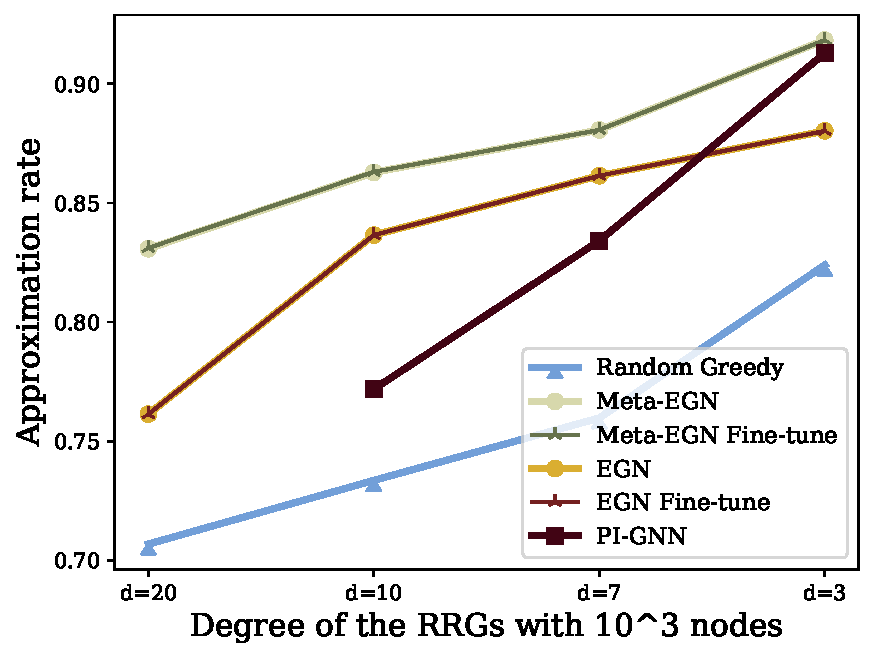
\includegraphics[width=0.32\textwidth]{iclr2023/img/exp/mis_10_3_ga.pdf}
         %\vspace{-0.6cm}
         %\caption{Performance on $10^3$ nodes}
         %\label{fig:mis_ga_103}
     %\end{subfigure}
     \hfill
     %\begin{subfigure}[c]{0.31\textwidth}
         %\centering
         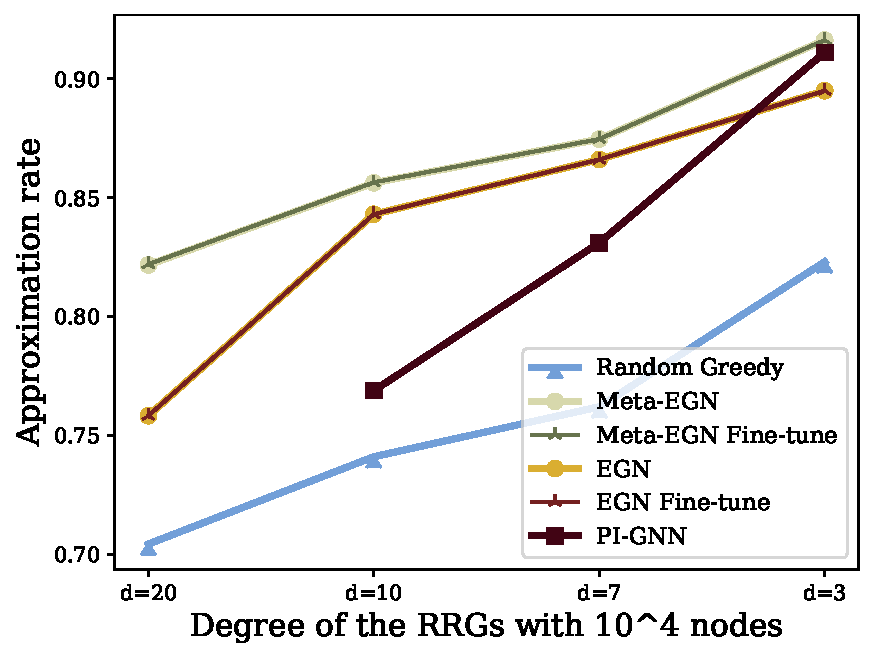
\includegraphics[width=0.32\textwidth]{iclr2023/img/exp/mis_10_4_ga.pdf}
         %\vspace{-0.6cm}
         %\caption{Performance on $10^4$ nodes}
        % \label{fig:mis_ga_104}
     %\end{subfigure}
     \hfill
     %\begin{subfigure}[c]{0.31\textwidth}
         %\centering
         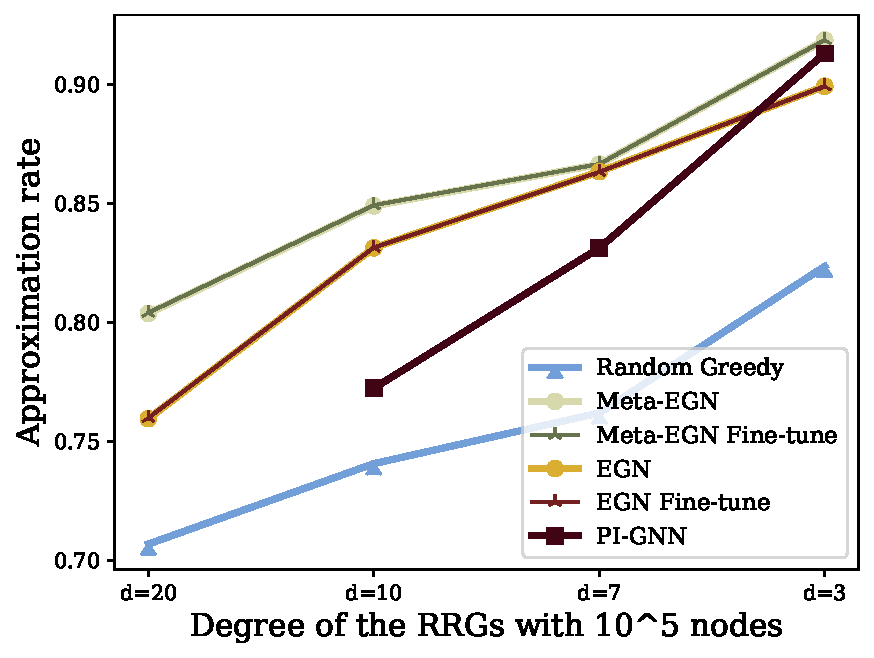
\includegraphics[width=0.32\textwidth]{iclr2023/img/exp/mis_10_5_ga.pdf}
         %\vspace{-0.6cm}
         %\caption{Performance on $10^5$ nodes}
         %\label{fig:mis_ga_105}
     %\end{subfigure}
     \vspace{-0.3cm}
        \caption{ApRs in the MIS problem on RRGs. %\proj and EGN are only trained on RRGs with $1000$ vertices and degrees randomly sampled from $3,7,10,20$. 
        Meta-EGN and EGN are both trained with the output of Random Greedy Algorithm (RGA) as initialization.}
        \label{fig:mis_ga}\vspace{-0.3cm}
\end{figure}


\subsection{\proj boosts the performance with distribution shifts}\label{sec:out-dis}
\textbf{Problem Scale Shift:} Here, we use large-scale RB graphs of 1000-5000 nodes to test EGN and \proj that is trained based on RB500. Table~\ref{tab:mc_generaliztaion_scale} shows the results. Both methods show good generalization while \proj is always better. As the scale increases, Meta-EGN outperforms Gurobi9.5. For example, it takes Meta-EGN with $4$ random initializations only $1.02$s to beat Gurobi9.5 that runs for $3000$ seconds on RB5000 dataset in the MC problem. Moreover, \proj can even outperform Gurobi9.5 on the MVC problem when the problem scale becomes large.

%Meta-EGN improves EGN especially in `Fast' and `Medium' cases with fewer number of random initializations.

%\textbf{Across Scale Generalization:}
%The generalization performance of EGN, Meta-EGN and Gurobi9.5 on extreme hard ($\rho = 0.25$) RB datasets  with vertices ranging from $1000$ to $5000$ of the MC problem are shown in Table~\ref{tab:mc_generaliztaion_scale} and the MVC problem in Table~\ref{tab:mvc_generaliztaion_scale}. The models are only pre-trained on training data with $500$ vertices. Both the unsupervised learning frameworks show good generalization ability with respect to scale changes, Meta-EGN improves EGN especially in `Fast' and `Medium' cases with fewer number of random initializations.
%As the scale increases, Meta-EGN outperforms Gurobi9.5. For example, it takes Meta-EGN with $4$ random initializations only $1.02$s to breakthrough the performance of Gurobi9.5 that has been running for $3000$ seconds on RB5000 dataset in the MC problem.

\textbf{Real-Synthetic Distribution Shift:} Here, we train EGN and \proj on Twitter and test them on RB500.  Table~\ref{tab:generalization_real_synthetic} shows the results. Compare Table~\ref{tab:generalization_real_synthetic} with Tables~\ref{tab:mc_performance},\ref{tab:mvc_performance}. We observe better generalization performance of \proj compared to EGN. For example, for the MC problem, \proj has almost the same performance 
whether there is a dataset shift or not (0.833 v.s. 0.834 before fine-tuning, 0.876 v.s. 0.878  after fine-tuning) while EGN has a bigger gap in performance when there is a shift (0.819 v.s. 0.829 before fine-tuning, 0.831 v.s. 0.864 after fine-tuning). For the MVC problem, although the performance drop of \proj is larger, such a drop is still much smaller than that of EGN.   

%When changing the data distribution, the Meta-EGN models merely pre-trained on source data distribution largely outperform EGN and could even achieve comparable performance with Gurobi9.5, showing its improvement in cross-distribution generalization.

\subsection{Max Independent Set: A response to~\citep{angelini2022cracking}}\label{sec:MIS}


\begin{wrapfigure}{r}{0.38 \linewidth}
\vspace{-7mm}
         \centering
         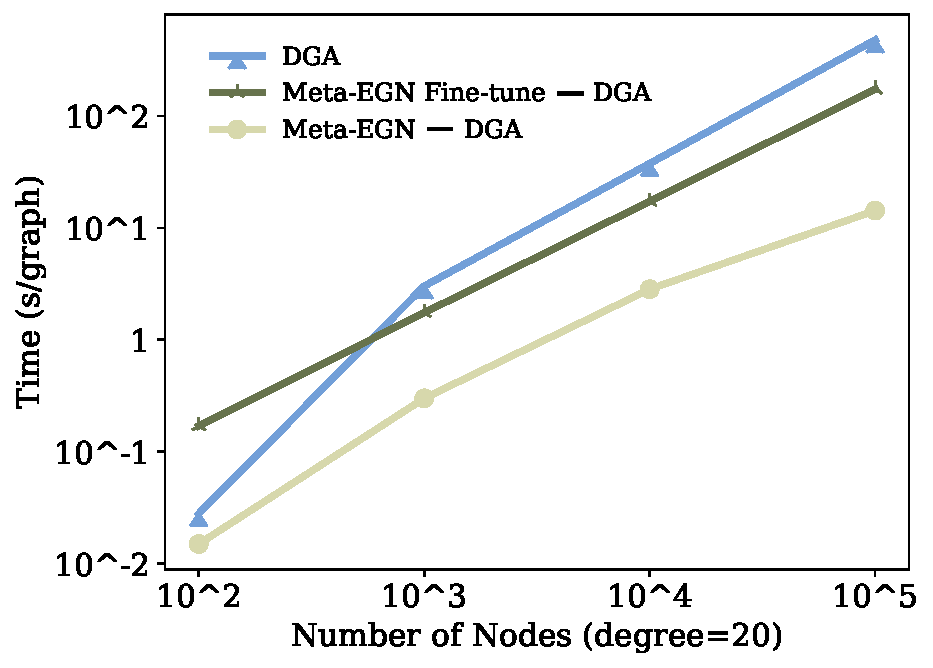
\includegraphics[width=0.38\textwidth]{iclr2023/img/exp/time_20.pdf}
         \vspace{-0.6cm}
         \caption{Time cost v.s. Graph  Scales.}
         \vspace{-0.3cm}
         \label{fig:mis_time}
\end{wrapfigure}


For the MIS problem on large-scale RRGs, ~\cite{angelini2022cracking} have recently posted a concern on learning-based methods by arguing that PI-GNN in~\cite{schuetz2022combinatorial} could not achieve comparable results with the heuristic algorithm DGA~\citep{angelini2019monte}. We see the reason comes from improper usage of learning-based methods in~\cite{schuetz2022combinatorial} as stated in Sec.~\ref{sec:intro}: 1) PI-GNN is trained directly on each single testing instance without learning from the training dataset that contains varies graphs, which is likely to be trapped into the local optima; 2) GNN generally suffers from a node ambiguity issue on RRGs. To resolve the problem, we utilize the outputs of DGA and RGA as the initialization of GNN inputs (EGN, \proj) and expect to learn heuristics from historical data to further tune the solutions given by the greedy algorithms. We train GNN models on RRGs with 1000 nodes with node degrees randomly sampled from $3,7,10,20$, and test on larger RRGs (up to $10^5$ nodes). %To the best of our knowledge, there exists no other non learning-based fine-tuning heuristics that further improves the greedy algorithms for MIS. 
Experiments show that \proj can further improve DGA (in Fig.~\ref{fig:mis}) and RGA (in Fig.~\ref{fig:mis_ga}), while EGN fails to better tune DGA. Note that here EGN and \proj adopt the exactly same backbones. We attribute the improvement to meta-learning-based training as adopted by \proj. See Table~\ref{tab:mis_statistics} in Appendix for more details of the numerical improvement by \proj. We also see in these cases, one-step fine-tuning does not contribute much to the performance of EGN or Meta-EGN, %(i.e. fine-tuning would increase the solution node number by $1$ for every $5$ graphs with degree $20$ and $10^5$ nodes), 
indicating the model before fine-tuning has been very close to a local minimum.

We also check the extra time cost by running \proj to improve DGA solutions in Fig.~\ref{fig:mis_time} and Fig.~\ref{fig:mis_time_app} in Appendix. The extra time cost is just 1\% (without fine-tuning) - 30\% (with fine-tuning) of the time cost of DGA. In theory, the extra time cost without fine-tuning should be $O(|E|)$ for GNN inference plus $O(|V|)$ for rounding, which is in the same order as DGA, while the GNN parallel inference substantially reduces the time.      

%(See Fig.~\ref{fig:mis})(See Fig.~\ref{fig:mis_ga})

%~\cite{angelini2022cracking} have posted a concern that the learning-based method in ~\cite{schuetz2022combinatorial} could not achieve comparable results with the degree-based greedy algorithm (DGA)~\citep{angelini2019monte} in the max independent set (MIS) problem on large scale random regular graphs (RRGs). The reason could be summarized from two aspects: 1) ~\cite{schuetz2022combinatorial} train and test on the same single graphs, which not only requires much time workload given a new testing graph but also makes no use of the heuristics from historical graphs. Thus we pre-train our Meta-EGN on randomly generated datasets with $1000$ vertices for a good initialization, then we either fine-tune the model in one-step or directly infer for time-complexity balance. The time-scale relation is shown in Fig.~\ref{fig:mis_time}, Using GNNs to infer would remain the same time complexity as pure DGA algorithms. 2) The GNNs' limited expressive power~\citep{xu2019powerful} would suffer from severe node ambiguity issue on regular graphs. To resolve the problem, we utilize the output of DGA (See Fig.~\ref{fig:mis}) or GA (See Fig.~\ref{fig:mis_ga}) as the initialization of GNN inputs and expect to learn heuristics to further modify the solution of the greedy algorithms. To the best of our knowledge, there exists no other non learning-based fine-tuning heuristics that further improves the greedy algorithms for MIS. Experiments show that Meta-EGN could improve the performance of both the DGA and GA initialization, while EGN could not outperform DGA even with the DGA initialization. 

%\hl{unfinished}











\iffalse
\subsubsection{max clique:} twitter, collab, IMDB, rbtest, rb500hard, rb1000hard
\subsubsection{vertex covering:} twitter, collab, IMDB, rb500hard, rb1000hard
\pan{I feel that it would be good to have one more setting}
\subsection{Meta brings higher generalization ability}
\subsubsection{from twitter to rb500hard}
max clique + vertex cover
\subsubsection{from rb500 to twitter}
max clique + vertex cover
\subsubsection{Different testing size trained on RB500}
max clique, vertex cover to rb1000hard, rb2000hard
\subsubsection{Different testing difficulty trained on RB500}
max clique, vertex cover
\subsubsection{Real dataset (twitter to other three)}
\subsection{Response to cracking: Meta has the potential to outperform simple baselines}
\hl{unfinished: large scale graphs}
The two charts between nature and cracking

\subsection{Ablation}
\hl{this part is unfinished? (low priority)}
\subsubsection{inner learning rate}
\subsubsection{batch size}



\begin{table}[]
\centering
\fontsize{8}{8}\selectfont
\setlength\tabcolsep{3pt}
\begin{tabular}{@{}ccccccc@{}}
\toprule
\multirow{}{}{} & \multicolumn{2}{c}{COLLAB} & \multicolumn{2}{c}{IMDB} & \multicolumn{2}{c}{RBtest} \\ \cmidrule(l){2-7} 
 & Approximation Rate & Loss Value & Approximation Rate & Loss Value & Approximation Rate & Loss Value \\ \midrule
EGN & 0.980 ± 0.082 & 17.84 & 0.921 ± 0.212 & -12.20 & 0.768 ± 0.061 & 296 \\
Meta-EGN & \textbf{0.995 ± 0.030} & \textbf{-17.81} & \textbf{0.987 ± 0.059} & \textbf{-347.99} & \textbf{0.779 ± 0.065} & \textbf{92.91} \\ \bottomrule
\end{tabular}
\vspace{-0.3cm}
\caption{Twitter to COLLAB, IMDB, RBtest performance on the max clique (MC) problem.}
\vspace{-0.6cm}
\label{tab:generalization_real_real}
\end{table}
\fi
